\chapter{Breve reseña de la Gestión de Casos}
\label{BPM}
%\section{Breve reseña de la Gestión de Casos}

La administración de los procesos ha sido una preocupación constante de los investigadores que han estado en la búsqueda de la optimización de los mismos, específicamente del flujo de los procesos conocido como \textit{Workflow}, para proporcionar mayor eficiencia a las empresas que los ejecutan. Se encuentra en \citet{van2005case} una revisión juiciosa de sistemas que administran los flujos de los procesos, y cómo, desde las fechas en que se proponen, en general, del siglo pasado, se diseñan modelos que permiten la flexibilidad de los mismos, atendiendo a las características dinámicas que han presentado los procesos y que hoy sigue ocupando a la comunidad científica. En este aparte se revisan técnicas de Inteligencia Artificial para establecer su aplicación en la adaptación de los BPMS ante la incertidumbre en los procesos.

El término Proceso de Negocio o BP (\textit{Business Process}) se refiere al conjunto de actividades que se ejecutan dentro de un proceso, en un orden determinado y de acuerdo a unos eventos iniciales. Así mismo, la Gestión de Procesos de Negocio o el BPM (\textit{Business Process Management}), viene gestionando estos procesos de negocios, mediante suites llamadas BPMS, que integran un conjunto de facilidades tecnológicas para el dueño del negocio. 

Varias de las funcionalidades con que cuentan las BPMS han sido mejoradas en los últimos años con la ayuda de técnicas de Inteligencia Artificial, para ofrecer mejor servicio a los clientes, acuñándose la sigla iBPM, que significa BPM Inteligente o iBPMS como sigla para las Suites o Sistemas para la Gestión de Procesos de Negocios Inteligentes.

Una BPMS se apoya en un conjunto de Reglas de Negocio - RN que contiene el conocimiento de los conocedores del negocio y que guían las decisiones en la ejecución de los procesos. En la mayoría de los casos se cuenta con un motor de RN que puede manejar las reglas en forma independiente de los procesos.

De otra parte, dado que los procesos de un negocio pueden ser dinámicos en el tiempo, se tiene la Gestión de Casos Adaptativos o \textit{ACM - Adaptive Case Management} \citep{pucher2010elements}, que pretende manejar la complejidad de los procesos donde no es fácil predecir el flujo de acciones o tareas que se requieren y en cuyas herramientas también se han vinculado técnicas de Inteligencia Artificial para lograr sus objetivos. 

Los casos, que se pretende apoyar con esta investigación, se definen en \citet{van2005case} como las situaciones que pueden ocurrir en el negocio y para las que no necesariamente se tienen predefinidos unos procedimientos a seguir. Allí se citan investigaciones basadas en Inteligencia Artificial que, es su momento, trabajaron en algoritmos de planificación y coordinación de procesos.

Para continuar con los antecedentes en BPM que permiten entender mejor el problema que apoya esta investigación, se revisó el cuadrante mágico de Garner de los \textit{iBPMS}, para establecer que Pegasystem, Appian e IBM son los fabricantes de suites más visionarios, que vienen liderando la oferta de servicios con mayor habilidad de ejecución, y que se plasma en la figura \ref{garner}. Las características inteligentes de estas tres suites se resumen en seguida.

\begin{figure}[htp]
	\centering
		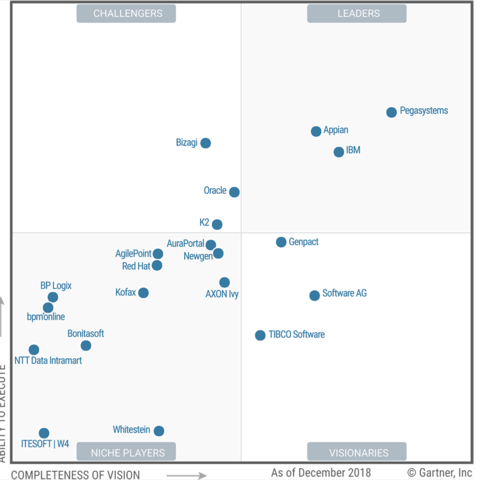
\includegraphics[scale=0.7]{Cuadrante magico 2018.png}
	\caption[Garner iBPMS 2019 ]{Cuadrante mágico de Garner para Suits de Gestión de Procesos de Negocio Inteligentes 2019}
	\label{garner}
\end{figure}

Pegasystem da uso a las tecnologías de la inteligencia artificial permitiendo a las empresas predecir el comportamiento de sus clientes para mejorar sus resultados. Además, refiere que ofrece soluciones inteligentes en BPM que incluye administración de casos, reglas de negocios y desarrollo de aplicaciones móviles, entre otras funcionalidades \citep{Pega2013}.

\citet{IBMKnowledgeCenter2017} muestra su inteligencia con IBM BPM Advancer, con la cual ofrece a las empresas la facilidad de la Gestión de Casos, mediante el aplicativo Basic Case Management, donde se tiene en cuenta lo impredecible de la secuencia de actividades en la gestión de casos y da las instrucciones al dueño del negocio para hacer uso de esta funcionalidad. Adicionalmente, cuenta con la herramienta IBM Watson que brinda funcionalidades de inteligencia artificial a las empresas, entre las que se cuenta el aprendizaje dinámico \citep{IBMSaladePrensa2017}.

Appian a su vez, expone que, mediante el Aprendizaje de Máquina, las BPMS están actuando sobre los grandes volúmenes de datos con que cuentan las empresas gracias al Internet de las Cosas; de aquí se descubren los gustos y tendencias de los clientes y con ello se apoya la toma de decisiones de las empresas; muestra la aplicación del Aprendizaje de Máquina en la automatización de procesos como una tendencia futura \citep{Potrzeba2016}. Algunas de las facilidades que ofrece la BPMS Appian son relacionadas por \citet{AlarconMatta2007},  así: gestión de documentos, gestión del contenido, herramientas de colaboración y soporte a comunidades de conocimiento. 

Así, se aprecia que, en los últimos años, las BPMS han desarrollado facilidades que involucran técnicas de inteligencia Artificial o Machine Learning, para brindar un servicio más eficiente a las empresas que deben lidiar con procesos altamente dinámicos. 

De otra parte, Business Process Model and Notation (BPMN) y Case Management Model and Notation (CMMN) son estándares para el modelado de procesos; el primero modela procesos estáticos y el segundo procesos dinámicos o Casos. De acuerdo con \citet{auer2014business}, estas notaciones deben combinarse para atender los requerimientos cambiantes de los negocios aprovechando la simplicidad del BPM.

El Aprendizaje Automático o \textit{Machine Learning} es una de las áreas de la Inteligencia Artificial que ha permitido un manejo eficiente de la información, teniendo en cuenta el volumen de datos que cada día se manejan en los negocios y en el mundo en general, apoyada en diferentes técnicas como las redes Neuronales, los Algoritmos Genéticos, las Colonias de Hormigas y el Soporte de Máquina Vectorial, entre otras. Técnicas como estas se vienen aplicando desde las investigaciones en los Workflow, como la referenciada por \citet{herbst2000machine} quienes aplican técnicas de Machine Learning a los grafos de los procesos e implementan técnicas de inferencia gramatical que están restringidas a flujos de trabajo secuenciales en Worflow concurrentes, dejando abierta la investigación para otros interesados. 
